\section{Introdução}\label{sec:intro}

\indent A agricultura brasileira desempenha um papel estratégico na economia nacional, sendo responsável por aproximadamente 23,2\% do Produto Interno Bruto (PIB) em 2024 \cite{cna2025}. No DF, em 2024, segundo dados de Dataviva, cerca de 21\% das exportações estaduais foram produtos agrícolas \cite{dataviva-graph-2025}; uma participação econômica significativa, possivelmente apontando que uma otimização do modelo de produção adotado poderia beneficiar não só os produtores, mas o restante da sociedade. A figura \ref{fig:dfexp} apresenta as exportações econômicas do Distrito Federal de forma gráfica para melhor análise.

\begin{figure}[!htpb]
    \centering
    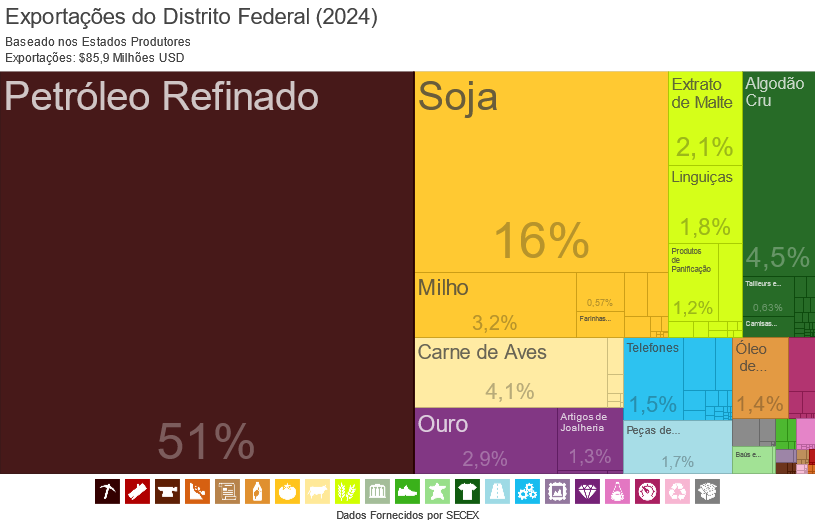
\includegraphics[width=.9\columnwidth]{figuras/expdf_area.png}
    \caption{Adaptado de Dataviva (2025)~\cite{dataviva-graph-2025}.}
    \label{fig:dfexp}
\end{figure}

% reescrito em 05092025 
Segundo a revisão bibliográfica realizada por Tschiedel e Ferreira, a agricultura de precisão é uma filosofia de gerenciamento de um campo agrícola que busca otimizar a produção utilizando sensores para obter dados sobre o clima e a terra e subsequentemente aumentar a capacidade do admnistrador de aplicar os insumos de forma correta, ou seja, onde são mais necessários para sustentar a produção \cite{tschiedel_ferreira_2002}. A partir dessa definição, é possível correlacionar o entendimento do clima de uma determinada região.

Uma breve pesquisa acerca das propostas do mercado para a obtenção de leituras meteorológicas locais revela que as soluções de estante tem um grande enfoque na obtenção dos dados, todavia falhando em prover análises mais detalhadas de possíveis mudanças temporais ou emitir alertas para seus usuários, apresentando um vácuo tecnológico capaz de ser explorado. A solução mais comum encontrada pela equipe pode ser exemplificada pelo modelo FT0350 da Gevanti \cite{FT0350}, uma estação meteorológica que possui sensores para coleta de dados e um display para apresentação dos dados imediatamente coletados, todavia carece de uma forma de reter esses dados e analisá-los.

O objetivo do trabalho apresentado por meio desse relatório é o projeto e execução de um protótipo de sistema computacional integrado com sensores capazes de prover análises simples para seu usuário utilizando técnicas de machine learning, tais como redes neurais. Em outras palavras, este trabalho propõe o desenvolvimento de uma estação meteorológica compacta para os fins de coleta e análise de dados, capaz de comunicar ao usuário final do sistema possíveis alertas e resultados. Além de já demonstrar resultados em outras áreas, segundo a revisão bibliográfica realizada por Benos et. al., redes neurais aplicadas a um ambiente rural aparentam ser um tópico em constante progresso \cite{machine_learning_in_agriculture}, permitindo uma oportunidade de estudo de vantagens e dificuldades apresentadas durante o desenvolvimento do sistema pretendido.

Para esse fim, será utilizado o SoC (System on a Chip) Raspberry Pi 3 Modelo B \cite{rpi3} e sensores específicos a serem detalhados posteriormente na lista de materiais, capazes de coletar dados climáticos e ambientais voltados para a aplicação agrícola. Além disso, o sistema incorpora um modelo de inteligência artificial que processa os dados localmente e envia os resultados para um servidor local, possibilitando a visualização em dashboards interativos.

\begin{figure}[!htpb]
    \centering
    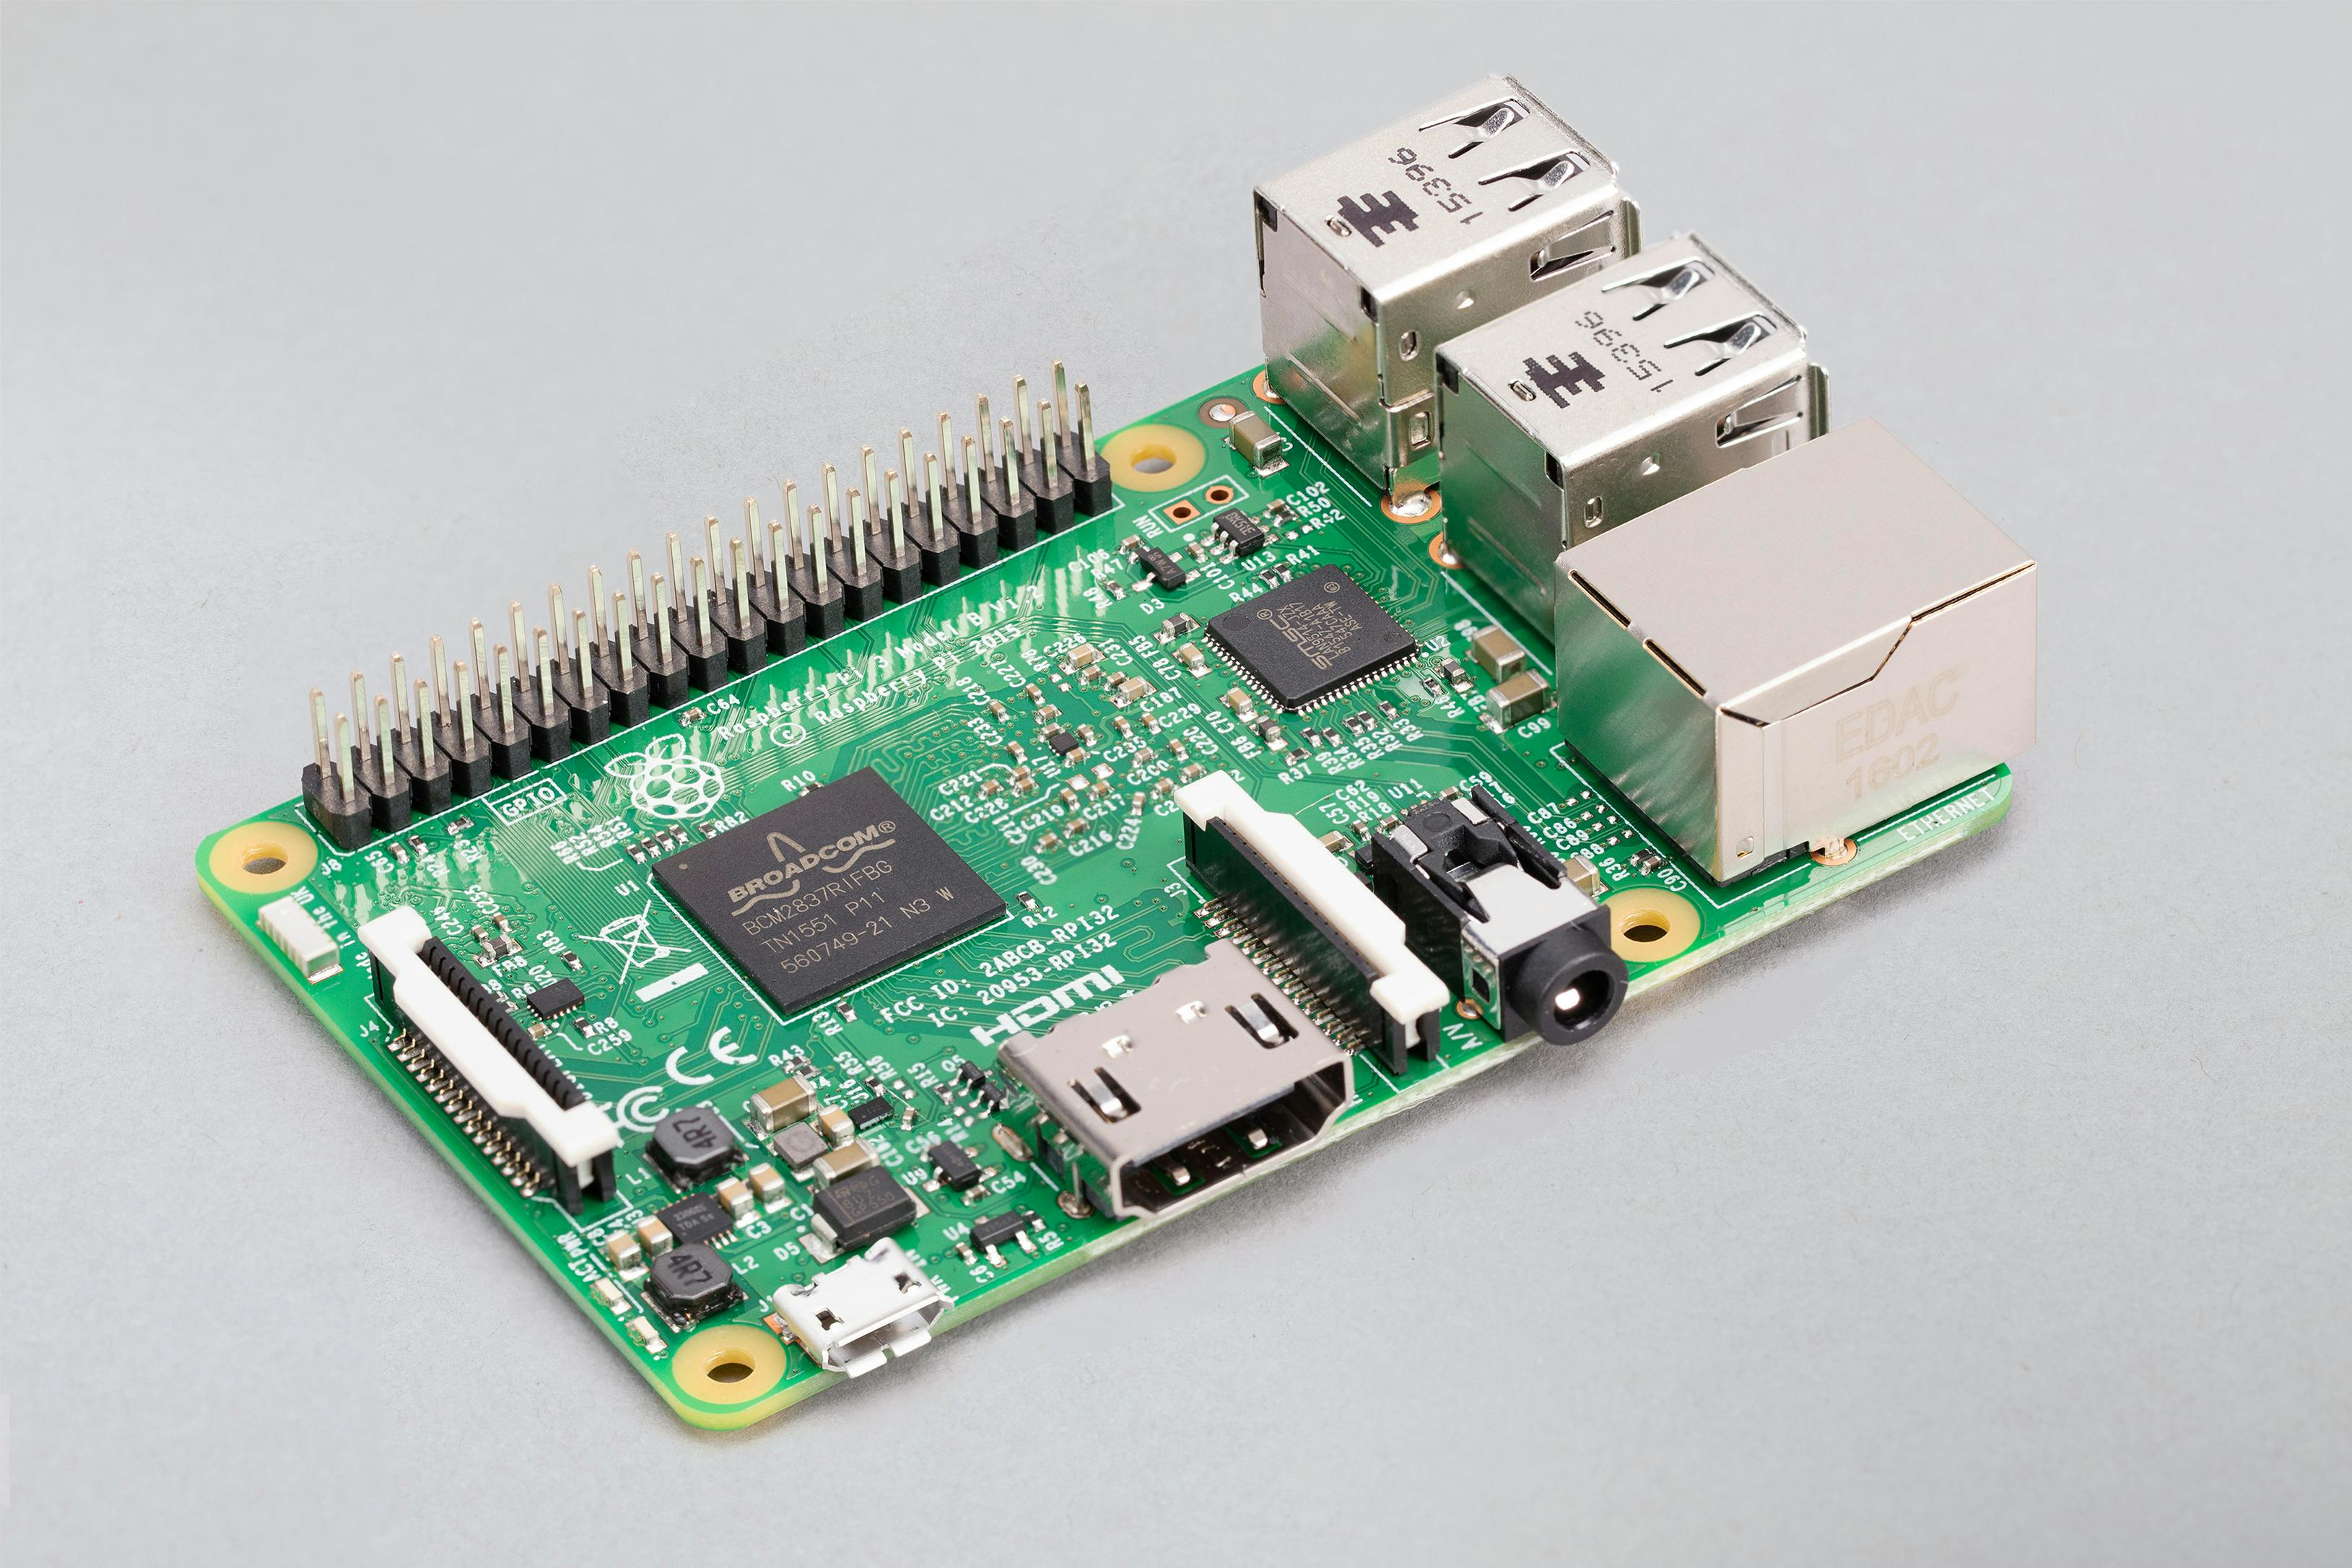
\includegraphics[width=.9\columnwidth]{figuras/rpi3.jpg}
    \caption{Raspberry Pi 3 Modelo B~\cite{rpi3}.}
    \label{fig:rpi3}
\end{figure}

\newpage

% Este documento \LaTeX~foi organizado em uma série de arquivos separados para cada Seção, localizados na pasta \texttt{editaveis}. 
% Confira ao longo dos arquivos como incluir
% figuras como a Fig. \ref{fig:rpi3}, além de tabelas, notas de rodapé e referências.
% Para acrescentar referências, altere o arquivo \texttt{editaveis/refs.bib}, que segue o formato BibTeX~\cite{ref:bibtex}. 

% Para manter o projeto organizado, acrescente suas figuras à pasta \texttt{figuras}. 
% % Confira no arquivo \texttt{editaveis/02\_introducao.tex} como incluir figuras como a Fig. \ref{fig:rpi3} e tabelas como a Tabela \ref{tab:pontuacao}.
% Para figuras e tabelas, não se preocupe com o posicionamento delas no texto. 
% O importante é que todas sejam referenciadas, assim como foi feito na segunda linha deste parágrafo.

% Todo o texto deve ser auto-contido; isto é, ele deve se explicar por si só. As figuras e tabelas somente \textit{auxiliam} no entendimento do texto. Sempre que o autor tiver que se explicar após a escrita, isto significa que o texto não está claro.

% O projeto completo deverá ser desenvolvido em ambiente Git público (GitHub, GitLab etc.), incluindo cronograma do projeto, código-fonte, código \LaTeX~deste relatório e resultados (planilhas, fotos etc).
% O repositório do projeto terá dois propósitos: servir de portfólio para os integrantes do grupo, e estender os conhecimentos de sala de aula para a comunidade em geral (créditos de extensão).


